\documentclass[tikz,border=10pt]{standalone}
\begin{document}
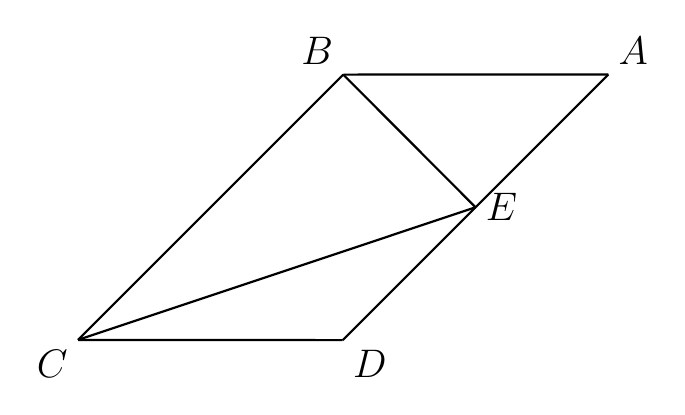
\begin{tikzpicture}[line join=round, line width=0.8pt]
\coordinate (A) at (3.374,1.701);
\coordinate (B) at (0.007,1.699);
\coordinate (C) at (-3.362,-1.670);
\coordinate (D) at (0.000,-1.673);
\coordinate (E) at (1.687,0.014);




\draw (B) -- (A);

\draw (A) -- (E) -- (D);

\draw (D) -- (C);

\draw (C) -- (B);

\draw (B) -- (E);
\draw (C) -- (E);


\node[above left, font=\fontsize{15}{18}\selectfont] at (B) {$B$};
\node[above right, font=\fontsize{15}{18}\selectfont] at (A) {$A$};
\node[right, font=\fontsize{15}{18}\selectfont] at (E) {$E$};
\node[below left, font=\fontsize{15}{18}\selectfont] at (C) {$C$};
\node[below right, font=\fontsize{15}{18}\selectfont] at (D) {$D$};
\end{tikzpicture}
\end{document}